% Chương 2: Cơ sở lý thuyết

\chapter{Cơ sở lý thuyết}

\label{Chapter2}

%----------------------------------------------------------------------------------------

\section{Mạng nơ-ron tích chập và học sâu}

\subsection{Tích chập hai chiều}

Phép tích chập là phép toán nền tảng trong CNN. Cho ảnh đầu vào $\mathbf{X} \in \mathbb{R}^{H \times W \times C}$ và bộ lọc (kernel) $\mathbf{K} \in \mathbb{R}^{k \times k \times C \times F}$, đầu ra của một lớp tích chập tại vị trí $(i, j)$ cho kênh đầu ra $f$ là:

\begin{equation}
    Y_{i,j,f} = \sum_{m=0}^{k-1} \sum_{n=0}^{k-1} \sum_{c=0}^{C-1} X_{i+m,\, j+n,\, c} \cdot K_{m,n,c,f} + b_f
    \label{eq:conv2d}
\end{equation}

trong đó $b_f$ là bias và $k$ là kích thước kernel. Sau tích chập, hàm kích hoạt ReLU thường được áp dụng: $\text{ReLU}(x) = \max(0, x)$.

\subsection{Batch Normalization}

Batch Normalization (BN) \cite{Goodfellow2016} chuẩn hóa đầu ra của lớp trước khi áp dụng hàm kích hoạt, giúp ổn định quá trình huấn luyện và cho phép sử dụng learning rate lớn hơn. Với mini-batch $\mathcal{B} = \{x_1, \ldots, x_m\}$:

\begin{equation}
    \hat{x}_i = \frac{x_i - \mu_{\mathcal{B}}}{\sqrt{\sigma_{\mathcal{B}}^2 + \epsilon}}, \qquad
    y_i = \gamma \hat{x}_i + \beta
    \label{eq:batchnorm}
\end{equation}

trong đó $\mu_{\mathcal{B}}$, $\sigma_{\mathcal{B}}^2$ là trung bình và phương sai của batch; $\gamma$, $\beta$ là tham số học được.

\section{Kiến trúc U-Net}

\subsection{Kiến trúc encoder-decoder}

U-Net \cite{Ronneberger2015} được Ronneberger và cộng sự đề xuất năm 2015, ban đầu cho bài toán phân đoạn tế bào kính hiển vi y tế. Kiến trúc bao gồm hai nhánh đối xứng:

\textbf{Encoder (đường giảm mẫu):} Gồm các khối DoubleConv lặp lại, mỗi khối gồm hai lớp tích chập $3 \times 3$ -- BatchNorm -- ReLU, theo sau là MaxPooling $2 \times 2$ để giảm không gian đặc trưng đồng thời tăng số kênh. Mạng đặc biệt trong đề tài này có encoder với bốn bước giảm mẫu, tăng số kênh từ 64 lên 128, 256, 512, rồi 1024.

\textbf{Decoder (đường tăng mẫu):} Sử dụng tích chập chuyển vị (transposed convolution) $2 \times 2$ để tăng gấp đôi không gian đặc trưng, sau đó nối (concatenate) với bản đồ đặc trưng tương ứng từ encoder qua skip connection, cuối cùng áp dụng DoubleConv.

\textbf{Skip connections:} Đây là đặc điểm then chốt của U-Net. Việc ghép nối trực tiếp bản đồ đặc trưng từ encoder sang decoder tương ứng giúp khôi phục chi tiết không gian bị mất trong quá trình giảm mẫu -- điều đặc biệt quan trọng với bài toán phân đoạn yêu cầu độ chính xác pixel.

Lớp đầu ra là tích chập $1 \times 1$ ánh xạ về số kênh bằng số lớp cần phân đoạn (ở đây là 1 cho bài toán phân đoạn nhị phân). Ngưỡng sigmoid $\sigma(\cdot) > 0.5$ xác định pixel là khối u.

Kiến trúc vanilla U-Net trong hệ thống BrainSeg-XAI được định nghĩa tại \texttt{models/unet.py} với các lớp: \texttt{inc}, \texttt{down1}--\texttt{down4}, \texttt{up1}--\texttt{up4}, \texttt{outc}.

\begin{figure}[h!]
    \centering
    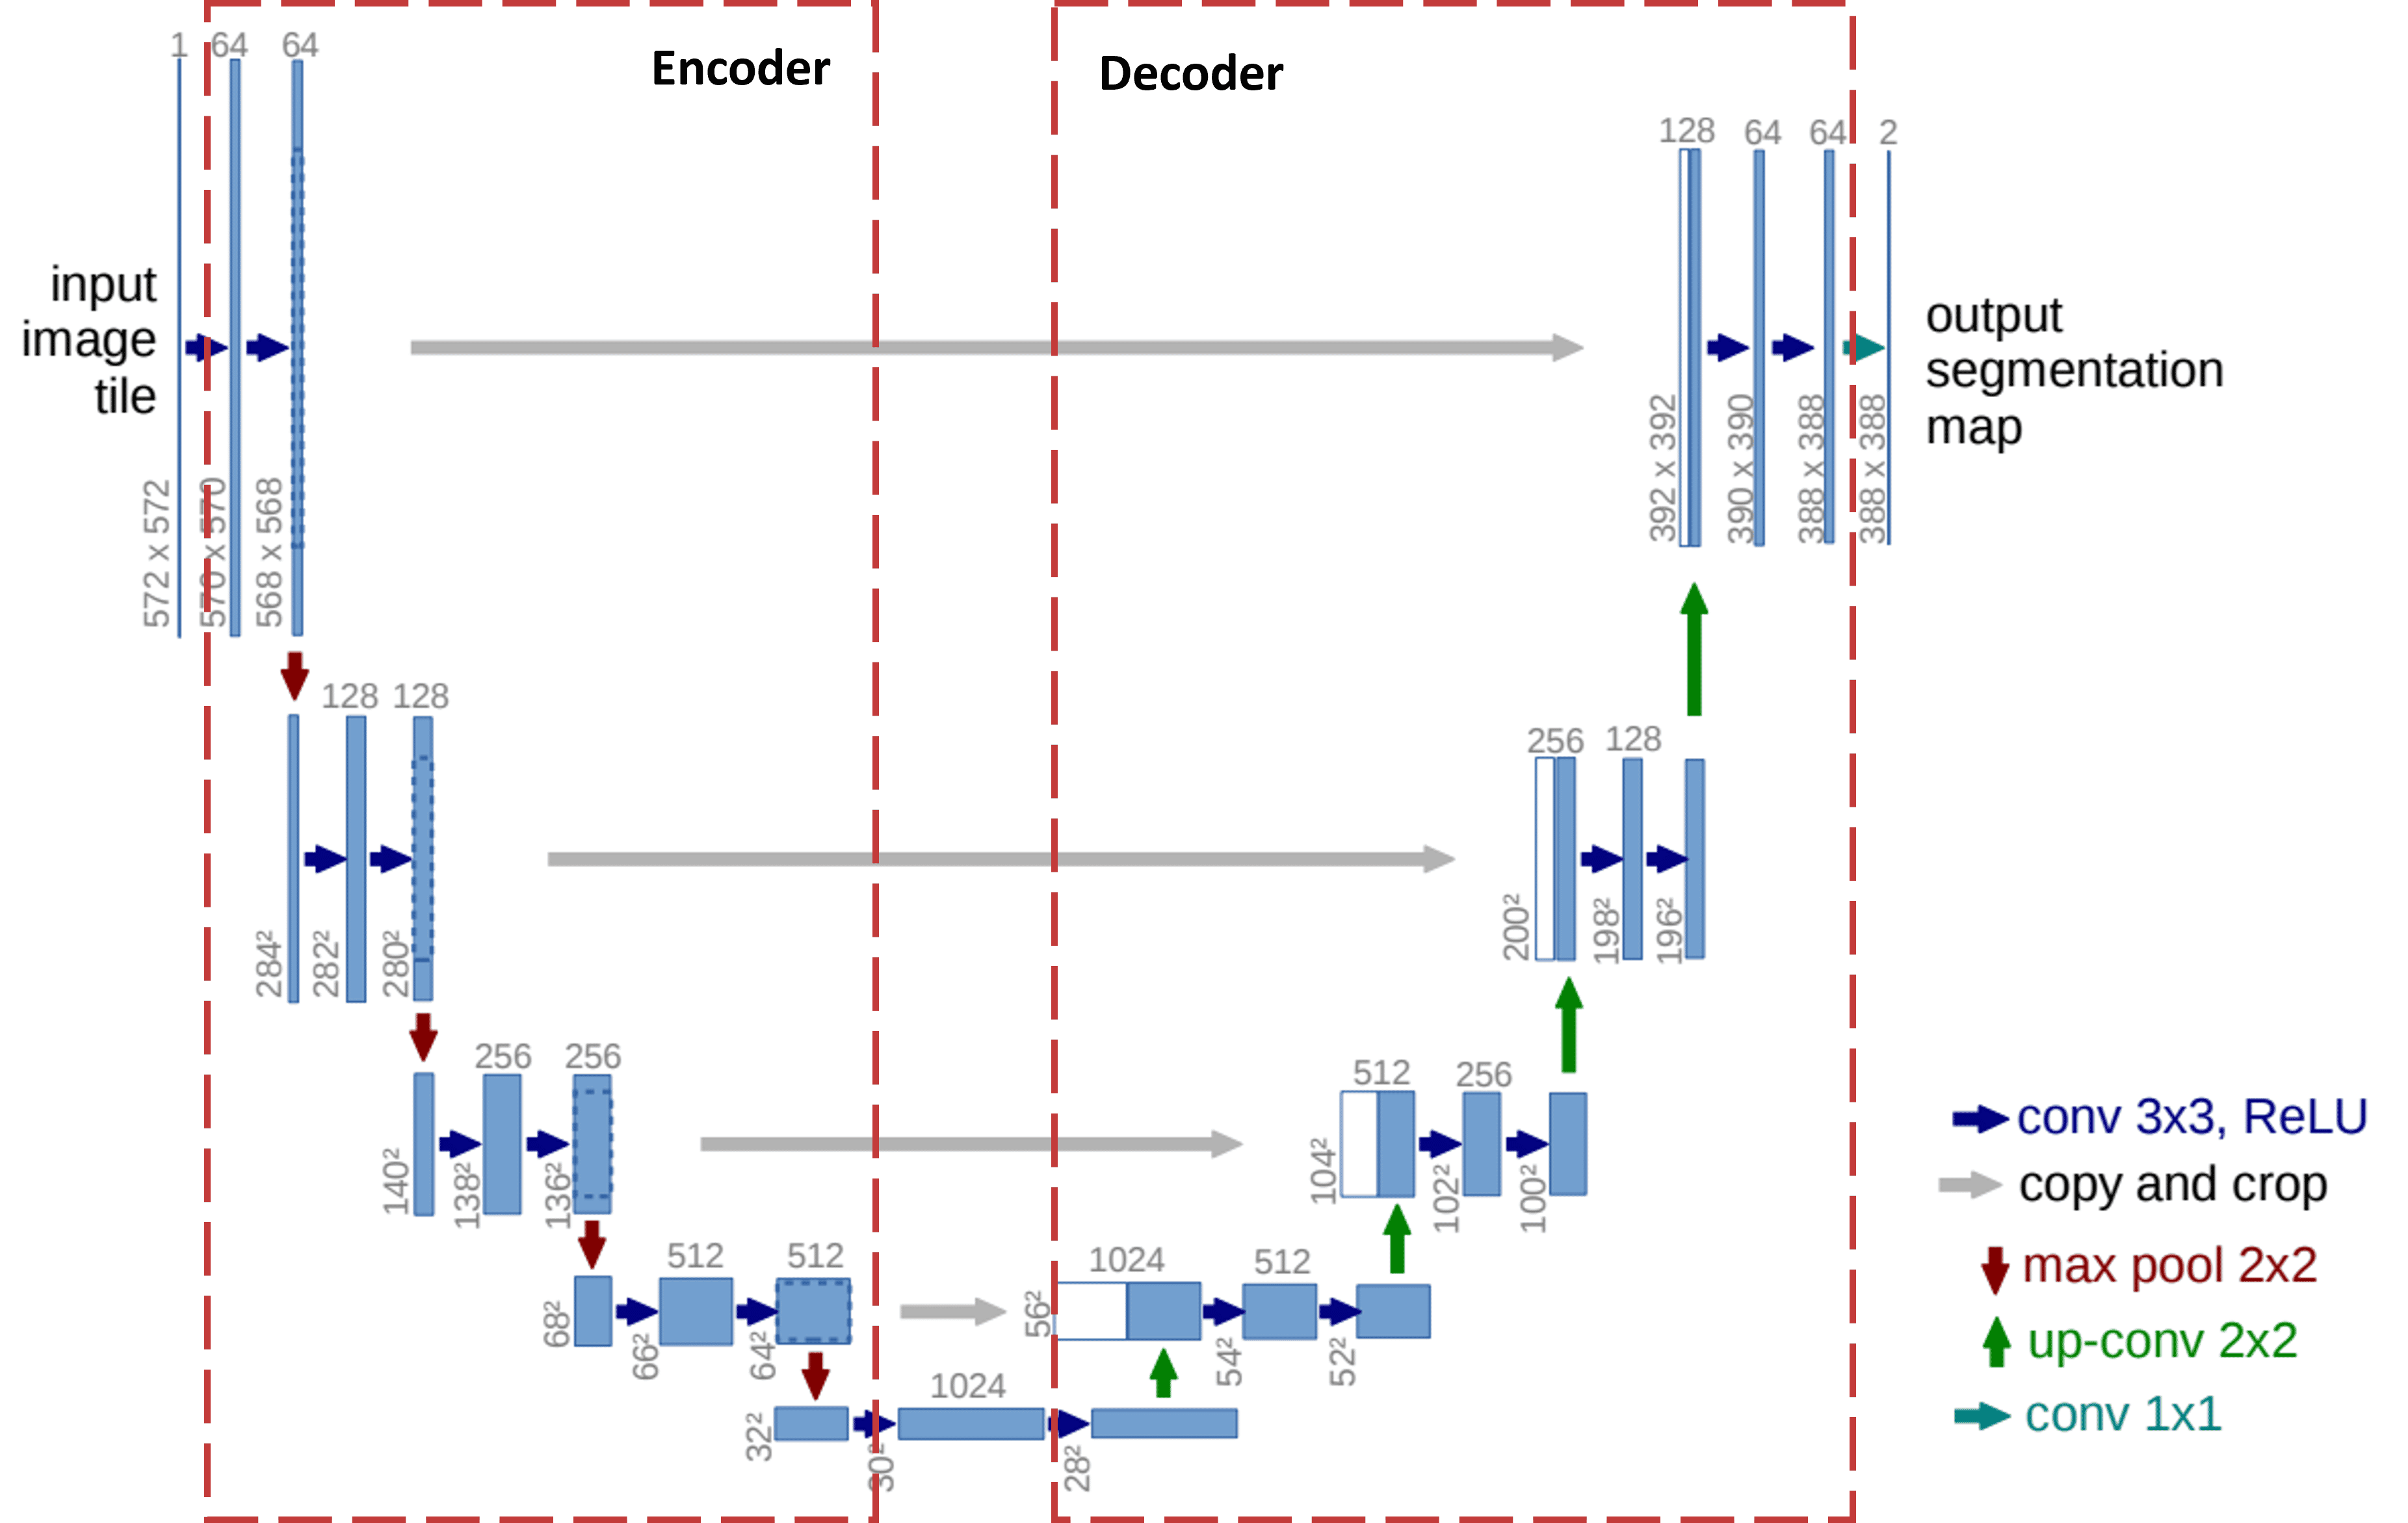
\includegraphics[width=0.88\textwidth]{Figures/Gallery/u-net.png}
    \caption{Kiến trúc U-Net: nhánh encoder giảm mẫu (trái) tăng số kênh đặc trưng, nhánh decoder tăng mẫu (phải) khôi phục độ phân giải không gian. Các mũi tên xám ngang biểu thị skip connections nối đặc trưng tương ứng từ encoder sang decoder.(Nguồn: \cite{Ronneberger2015})}
    \label{fig:unet_arch}
\end{figure}

\subsection{U-Net++}

U-Net++ \cite{Zhou2018} là phần mở rộng của U-Net, giới thiệu các nút trung gian $x^{i,j}$ trên các skip connections, trong đó $i$ là chỉ số độ sâu encoder và $j$ là chỉ số bước trong kiến trúc lồng nhau. Công thức tính nút trung gian:

\begin{equation}
    x^{i,j} = \mathcal{H}\!\left(
        \left[ x^{i,k} \right]_{k=0}^{j-1},\;
        \mathcal{U}(x^{i+1,j-1})
    \right)
    \label{eq:unetpp}
\end{equation}

trong đó $\mathcal{H}$ là khối tích chập dày đặc, $\mathcal{U}$ là phép tăng mẫu, và $[\cdot]$ là phép nối tensor. Mật độ kết nối cao hơn giúp U-Net++ khai thác thông tin đặc trưng ở nhiều tỷ lệ không gian, cải thiện đặc biệt với các cấu trúc có kích thước đa dạng.

Trong hệ thống BrainSeg-XAI, U-Net++ được khởi tạo qua thư viện SMP \cite{Yakubovskiy2019} với encoder EfficientNet-B4 \cite{Tan2019} pretrained trên ImageNet.

\begin{figure}[h!]
    \centering
    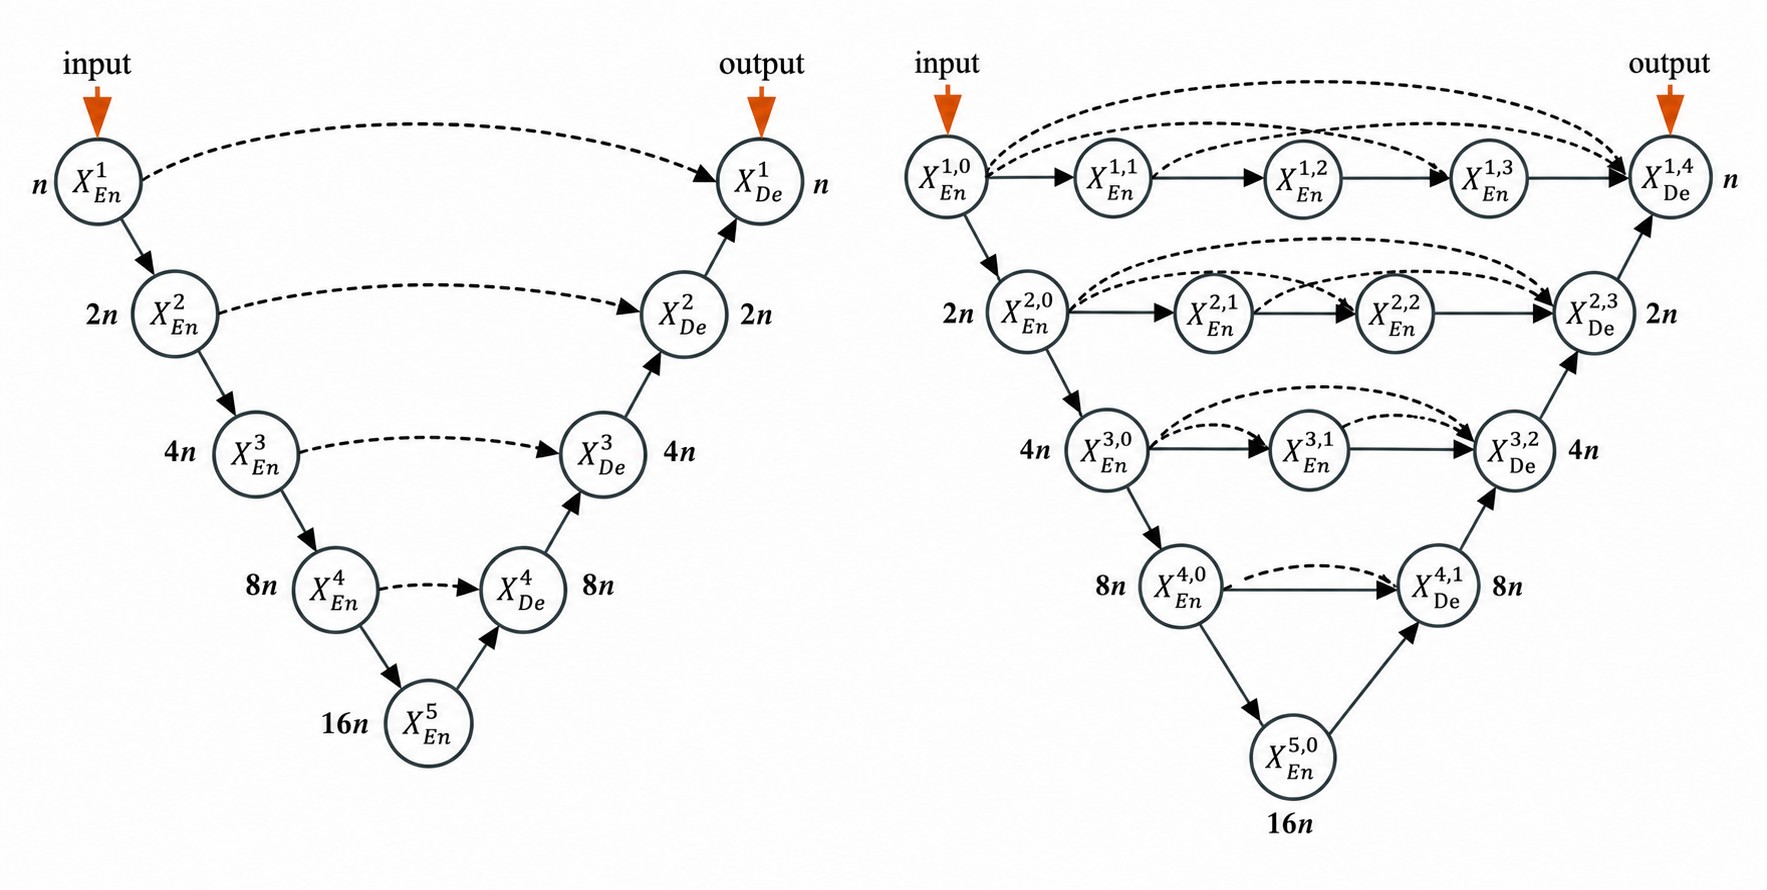
\includegraphics[width=0.82\textwidth]{Figures/Gallery/unet_vs_unetpp.png}
    \caption{So sánh đồ thị kết nối giữa U-Net (trái) và U-Net++ (phải). (Nguồn: \cite{Zhou2018})}
    \label{fig:unetpp_compare}
\end{figure}

\subsection{EfficientNet-B2 làm encoder}

EfficientNet \cite{Tan2019} sử dụng chiến lược ``compound scaling'' -- đồng thời tăng chiều rộng, chiều sâu và độ phân giải theo một hệ số $\phi$ -- để tối ưu hiệu quả tham số. EfficientNet-B2 với khoảng 19 triệu tham số cho hiệu suất cao trên ImageNet trong khi tiêu thụ ít tài nguyên tính toán hơn so với ResNet-50 hay VGG-16. Việc sử dụng encoder pretrained trên ImageNet giúp khởi tạo với các đặc trưng hình ảnh phong phú, quan trọng khi dữ liệu y tế thường hạn chế.

\section{Grad-CAM: Gradient-weighted Class Activation Mapping}

\subsection{Nguyên lý}

Grad-CAM \cite{Selvaraju2017} tính toán tầm quan trọng của mỗi kênh đặc trưng $k$ trong lớp tích chập mục tiêu bằng cách lấy trung bình toàn cục gradient của tín hiệu mục tiêu $y^c$ (đầu ra lớp cuối) theo bản đồ đặc trưng $A^k$:

\begin{equation}
    \alpha_k^c = \frac{1}{Z} \sum_i \sum_j \frac{\partial y^c}{\partial A_{ij}^k}
    \label{eq:gradcam_weight}
\end{equation}

trong đó $Z = H \times W$ là kích thước không gian của bản đồ đặc trưng. Bản đồ Grad-CAM sau đó được tính bằng tổ hợp tuyến tính có trọng số $\alpha_k^c$, áp dụng ReLU để giữ lại chỉ các ảnh hưởng tích cực:

\begin{equation}
    L_{\text{Grad-CAM}}^c = \text{ReLU}\!\left( \sum_k \alpha_k^c A^k \right)
    \label{eq:gradcam_map}
\end{equation}

Kết quả là bản đồ nhiệt có kích thước bằng bản đồ đặc trưng, sau đó được nội suy về kích thước ảnh gốc để trực quan hóa.

\subsection{Triển khai trong BrainSeg-XAI}

Module \texttt{xai/gradcam.py} đăng ký hai hook PyTorch tại thời điểm khởi tạo:
\begin{itemize}
    \item \texttt{register\_forward\_hook}: lưu bản đồ đặc trưng $A^k$ trong lượt truyền xuôi.
    \item \texttt{register\_full\_backward\_hook}: lưu gradient $\partial y^c / \partial A^k$ trong lượt truyền ngược.
\end{itemize}

\begin{sloppypar}
Lớp mục tiêu (\textit{target layer}) được chọn theo loại mô hình: \texttt{model.up4.conv.conv[-3]} cho vanilla UNet (lớp tích chập cuối trước lớp đầu ra); \texttt{model.segmentation\_head[0]} cho SMP (lớp tích chập đầu tiên trong segmentation head).
\end{sloppypar}

Tín hiệu mục tiêu là tổng toàn bộ đầu ra sigmoid: $y^c = \sum_{i,j} \sigma(\text{logit}_{ij})$, phù hợp với bài toán phân đoạn nhị phân nơi không có nhãn lớp đơn.

\section{Hàm mất mát cho phân đoạn nhị phân}

\subsection{Hệ số Dice}

Hệ số Dice đo lường mức độ chồng lấp giữa mặt nạ dự đoán $\hat{Y}$ và nhãn thực $Y$:

\begin{equation}
    \text{Dice}(\hat{Y}, Y) = \frac{2 \sum_{i} \hat{y}_i y_i}{\sum_{i} \hat{y}_i^2 + \sum_{i} y_i^2 + \epsilon}
    \label{eq:dice}
\end{equation}

trong đó $\epsilon$ là hằng số nhỏ để tránh chia cho 0. Hàm mất mát Dice: $\mathcal{L}_{\text{Dice}} = 1 - \text{Dice}$.

\subsection{Binary Cross-Entropy}

Hàm BCE đo lỗi pixel-level:

\begin{equation}
    \mathcal{L}_{\text{BCE}} = -\frac{1}{N} \sum_{i=1}^{N} \left[ y_i \log \hat{p}_i + (1 - y_i) \log(1 - \hat{p}_i) \right]
    \label{eq:bce}
\end{equation}

trong đó $\hat{p}_i = \sigma(\text{logit}_i)$ là xác suất dự đoán pixel $i$ là khối u. Trong thực tế huấn luyện, hàm mất mát kết hợp $\mathcal{L} = \mathcal{L}_{\text{BCE}} + \mathcal{L}_{\text{Dice}}$ thường cho kết quả tốt hơn từng thành phần đơn lẻ.

\section{Trích xuất đặc trưng hình thái học}

\subsection{Phân tích thành phần liên thông}

Hệ thống sử dụng \texttt{scipy.ndimage.label} để phân tách mặt nạ nhị phân thành các thành phần liên thông (connected components). Mỗi thành phần tương ứng với một vùng khối u riêng biệt.

\subsection{Các đặc trưng hình dạng}

\begin{sloppypar}
Trên vùng khối u lớn nhất (largest region), \texttt{skimage.measure.regionprops} cung cấp các thuộc tính sau:
\end{sloppypar}

\textbf{Độ bất đối xứng hình dạng (shape irregularity):}
\begin{equation}
    I_{\text{shape}} = 1 - \frac{4\pi A}{P^2}
    \label{eq:irregularity}
\end{equation}
trong đó $A$ là diện tích (pixel) và $P$ là chu vi. Phần tử $4\pi A / P^2$ chính là chỉ số compactness (nén tròn), bằng 1 khi vùng hoàn toàn hình tròn. Giá trị $I_{\text{shape}}$ cao cho thấy hình dạng bất quy tắc, thường liên quan đến khối u ác tính có ranh giới không đều.

\textbf{Độ phức tạp đường biên (boundary complexity):}
\begin{equation}
    B_c = \frac{P}{\sqrt{A} + \epsilon}
    \label{eq:boundary}
\end{equation}
Tỷ lệ chu vi trên căn bậc hai diện tích phản ánh mức độ gồ ghề của đường biên khối u. Giá trị lớn cho thấy đường biên phức tạp với nhiều lồi lõm.

\textbf{Dịch chuyển đường giữa (midline shift):}
\begin{equation}
    \text{shift} = \left| \frac{c_x}{W} - 0.5 \right| > 0.10
    \label{eq:midline}
\end{equation}
trong đó $c_x$ là tọa độ x tâm khối u và $W$ là chiều rộng ảnh. Dịch chuyển quá 10\% từ đường giữa là chỉ điểm lâm sàng quan trọng về tình trạng hiệu ứng khối.

\textbf{Chuyển đổi đơn vị diện tích:}
Giả sử lát cắt MRI tiêu chuẩn rộng 24 cm trên ảnh $256 \times 256$, hệ số chuyển đổi là $(24/256)^2 \approx 0.00879 \text{ cm}^2/\text{pixel}$.

\section{Hệ thống phân loại cấp độ nguy hiểm (Rule-based Risk Engine)}

\subsection{Thiết kế hệ thống}
Hệ thống cấp độ nguy hiểm được thiết kế theo nguyên lý \textit{additive scoring}: mỗi quy tắc cộng một điểm cố định vào điểm rủi ro tổng hợp $S_{\text{risk}}$, giới hạn tối đa 100. Thiết kế này cho phép truy vết nguyên nhân đóng góp vào điểm rủi ro cuối cùng. Sáu quy tắc hiện có:

\begin{table}[h!]
    \centering
    \caption{Các quy tắc trong bộ máy đánh giá rủi ro y khoa.}
    \label{tab:rules}
    \begin{tabular}{l l r}
        \toprule
        \tabhead{Quy tắc} & \tabhead{Điều kiện} & \tabhead{Điểm cộng} \\
        \midrule
        R1: Tỷ lệ chiếm diện tích   & occupancy $> 20\%$          & $+30$ \\
                                     & occupancy $> 10\%$          & $+20$ \\
                                     & occupancy $> 5\%$           & $+10$ \\
        R2: Bất đối xứng hình dạng  & irregularity $> 0.7$        & $+25$ \\
                                     & irregularity $> 0.5$        & $+15$ \\
        R3: Phức tạp đường biên     & boundary\_complexity $> 15$ & $+20$ \\
                                     & boundary\_complexity $> 10$ & $+10$ \\
        R4: Dịch chuyển đường giữa  & midline\_shift = True       & $+20$ \\
        R5: Số vùng khối u          & num\_regions $> 3$          & $+15$ \\
                                     & num\_regions $> 1$          & $+8$  \\
        R6: Diện tích tuyệt đối     & area $> 10$ cm²             & $+15$ \\
                                     & area $> 4$ cm²              & $+8$  \\
        \bottomrule
    \end{tabular}
\end{table}

\subsection{Phân loại mức rủi ro}

Bốn mức rủi ro được ánh xạ từ điểm số:

\begin{table}[h!]
    \centering
    \caption{Ánh xạ điểm rủi ro sang mức phân loại.}
    \label{tab:risktier}
    \begin{tabular}{l l l l}
        \toprule
        \tabhead{Mức rủi ro} & \tabhead{Khoảng điểm} & \tabhead{Mức độ} & \tabhead{Màu hiển thị} \\
        \midrule
        Thấp       & $0 - 29$  & Nhẹ       & Xanh lá  \\
        Trung bình & $30 - 49$ & Trung bình & Vàng  \\
        Cao        & $50 - 69$ & Nghiêm trọng & Cam  \\
        Rất cao    & $70+$     & Nguy kịch  & Đỏ \\
        \bottomrule
    \end{tabular}
\end{table}
